\documentclass[12pt, letterpaper]{article}
\usepackage{graphicx} % Required for inserting images

\usepackage{hyperref} % Better references
\renewcommand{\equationautorefname}{Eq.}  % Refer to equations as Eq.

\title{Sample Project}
\author{Ryan Draves}
\date{January 2025}

\begin{document}

\maketitle

\begin{abstract}
This is a sample document used to show Bazel Latex working. Most items in `class/` will be `.gitignored`'d as real assignments shouldn't be on a public repo.

The following is mostly stuff from the Overleaf \href{https://www.overleaf.com/learn/latex/Learn_LaTeX_in_30_minutes}{Learn LaTeX in 30 minutes} tutorial.

If one feels inspired to try this out, a simple way to get live updates is install node modules locally with \texttt{pnpm i} then run \texttt{npx ibazel run //class/sample:sample\_pdf} to see the changes in real time.
\end{abstract}

\section{Introduction}
\label{sec:intro}
First document. This is a simple example, with no
extra parameters or packages included.

Some of the \textbf{greatest} discovered in \textit{science} where made by \textbf{\underline{accident}}, such as in \autoref{fig:transfer}.

\begin{itemize}
    \item Item 1
    \item Item 2
\end{itemize}

\begin{enumerate}
    \item Item 1
    \item Item 2
\end{enumerate}

Simple equation $a^2 + b^2 = c^2$

\begin{equation}
    a^2 + b^2 = c^2
    \label{eq:py}
\end{equation}

\begin{figure}[t]
    \centering
    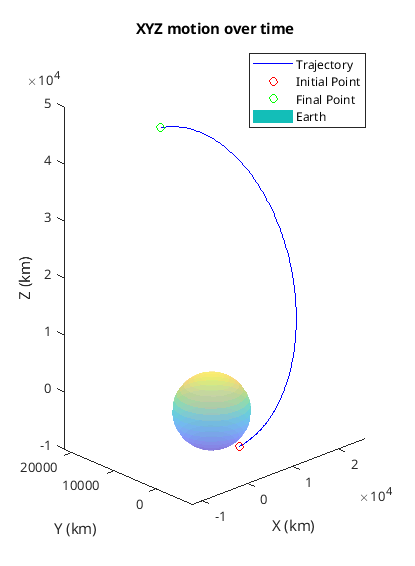
\includegraphics[width=0.5\linewidth]{transfer.png}
    \caption{Enter Caption}
    \label{fig:transfer}
\end{figure}

Subscripts in math mode are written as $a_b$ and superscripts are written as $a^b$. These can be combined and nested to write expressions such as

\[ T^{i_1 i_2 \dots i_p}_{j_1 j_2 \dots j_q} = T(x^{i_1},\dots,x^{i_p},e_{j_1},\dots,e_{j_q}) \]

We write integrals using $\int$ and fractions using $\frac{a}{b}$. Limits are placed on integrals using superscripts and subscripts:

\[ \int_0^1 \frac{dx}{e^x} =  \frac{e-1}{e} \]

Lower case Greek letters are written as $\omega$ $\delta$ etc. while upper case Greek letters are written as $\Omega$ $\Delta$.

Mathematical operators are prefixed with a backslash as $\sin(\beta)$, $\cos(\alpha)$, $\log(x)$ etc.

We can reference \autoref{table:1a} and \autoref{eq:py}. Both of these are found in \nameref{sec:intro}.

\begin{table}[h!]
\centering
\begin{tabular}{c|c}
    1 & 2 \\
    3 & 4
\end{tabular}
\caption{Sample caption}
\label{table:1a}
\end{table}

\end{document}
